\documentclass[12pt]{article}
\usepackage{amsfonts,amssymb}
\usepackage{amsmath}
\usepackage{amsthm}
\usepackage{hyperref}
\usepackage{graphicx}
\usepackage{listings}
%\documentstyle[12pt,amsfonts]{article}
%\documentstyle{article}

\setlength{\topmargin}{-.5in}
\setlength{\oddsidemargin}{0 in}
\setlength{\evensidemargin}{0 in}
\setlength{\textwidth}{6.5truein}
\setlength{\textheight}{8.5truein}
%
%\input ../adgeomcs/lamacb.tex
%\input ../mac.tex
%\input ../mathmac.tex
%
\input xy
\xyoption{all}
\def\fseq#1#2{(#1_{#2})_{#2\geq 1}}
\def\fsseq#1#2#3{(#1_{#3(#2)})_{#2\geq 1}}
\def\qleq{\sqsubseteq}
\newtheorem{theorem}{Theorem}
%cis51109hw1

%
\begin{document}
\begin{center}
\fbox{{\Large\bf Graph Theory}}\\
\vspace{1cm}
\end{center}

\vspace{0.5cm}\noindent


\section*{Graph isomorphism}

Let $G = (V, E)$ and $G'=(V',E')$. $G$ and $G'$ are isomorphic if there is a bijection $f: V \rightarrow V'$ such that for every pair of vertices $x, y \in V$, $(x, y) \in E$ if and only if $(f(x), f(y)) \in E'$. The function f is called an isomorphism from G to G'. 

\medskip

Another way of saying this is that $G$ and $G'$ are isomorphic if there is bijection between the vertex sets that preserves adjacency.

For an example, try an identify all pairs of isomorphic graphs in the following picture


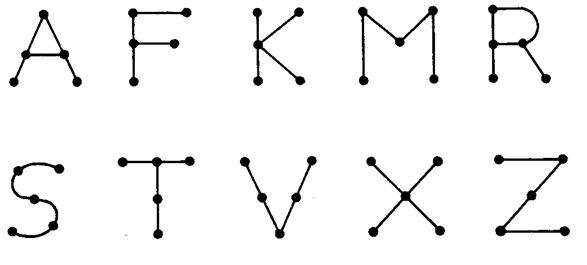
\includegraphics[scale=0.6]{./img/iso.jpg}

Graph isomorphisms are actually one of the hardest problems (more on this in 596) that computer science has.

Why is that the case?

Given an mapping that claims to be an isomorphism it is easy to check if it truly is one or not.

However, what if someone asks you to find such a mapping?

How many one-one and onto mappings are there between the two vertex sets? 

We know that if we have a bijection then the two vertex sets must have the same cardinality. So let us compute this in terms of $|V|$. We get $|V|!$. Obviously this is a function that grows really really fast so it is annoying to have to check all of these mappings.

There are certain tips that can help us detect whether two graphs could be isomorphic or not.

Here are some of them

\begin{itemize}
\item For obvious reasons, the two graphs have to have the same number of edges and vertices.
\item Under an isomorphism the degree of a vertex is preserved. So if the vertex $v$ had a degree of $k$ in graph $G$. Consider the isomorphism to be the function $f$. $f(v)$ which will be vertex in $G'$ must have the same degree $k$.
\item The degree sequence of two isomorphic graphs has to be the same. The degree sequence of a graph is a list of the degrees of all of the vertices in non-increasing order.
\end{itemize}

Here is an example of two non-isomorphic graphs which violate at least one of the properties above.

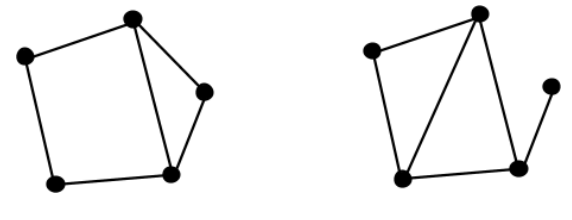
\includegraphics[scale=0.5]{./img/nonisodeg.png}


As an example here are two non-isomorphic graphs. They however are not violating any of the properties mentioned above

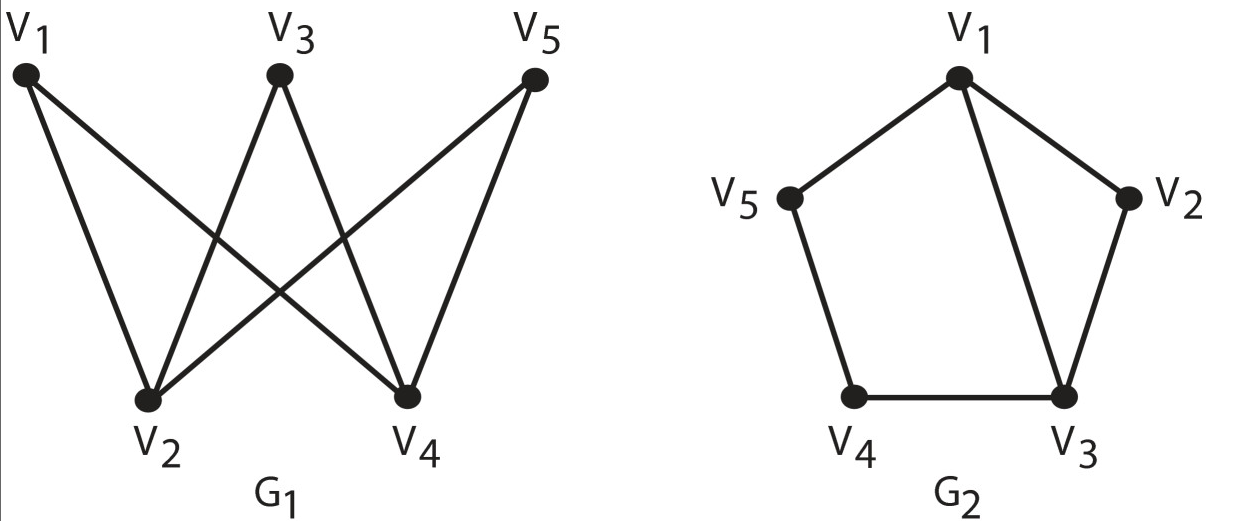
\includegraphics[scale=0.5]{./img/noniso.png}


\section*{Circuits and cycles}

A circuit is a walk in which the first vertex is the same as the last vertex. A sequence of one vertex, denoted $<a>$, is a circuit of length 0. Any circuit must have at least one repeated vertex because, by definition, the first and last vertices of a circuit are the same. A circuit is a cycle if it has length at least three and there are no additional repeated vertices, besides the first and the last. 

\section*{Connectedness and connected components}

A vertex v is said to be connected to vertex w in a graph G if there is a path in G from v to w. Since G is assumed to be undirected, a path from v to w implies that there is also a path from w to v. By definition, every vertex is connected to itself by a path of length 0. A vertex that is not connected with any other vertex is called an isolated vertex.

A graph is said to be connected if every vertex is connected to every other vertex in the graph and is disconnected otherwise. The property of being connected is a desirable property in many situations such as when the graph represents a road or communication network. If a graph is not connected, it has more than one connected component. 

\section*{Trees}

A connected acyclic (no cycles present) graph is called a tree. 

Trees are one of the fundamental structures in computer science. You will learn about them in data structures. You will also learn about them in algorithms.

Properties of trees

We can show the following property
 

\textbf{Result}

Every tree with at least one edge has a leaf (vertex of degree 1).

\vspace*{0.1in}

Proof.

We do this proof by providing a method to find a leaf.

Consider any vertex of the tree.  Find the longest path out of that vertex. 

Claim that this longest path will terminate in a vertex of degree 1. This claim can be proved based on the fact that trees are acyclic. Wherever the longest path ends, we cannot have an edge from that terminal vertex back to any of the other vertices in the path because that would create a cycle.

Therefore it must be the case that the last vertex on this longest path will be a leaf.


\textbf{Result}

In any tree $e = v - 1$.

Proof by induction on the number of vertices.

Base case. 1 vertex and no edge. Easy.

Assume it works for $k$ vertices. 

Consider a $k+1$ vertex tree.

It has a leaf because of the result above

Remove leaf and the one edge coming out of it.

We still have a connected acyclic graph (a tree).  So the induction hypothesis applies.

\textit{Finish the rest of this...}


\section*{Planar connected graphs}

Show that v - e + f = 2
 

\end{document}



